\section{Non-negativity and sums of squares} 

In this chapter, $n \in \N$ and  
\[
X=(X_1,\ldots,X_n)
\]
is a tuple of $n$ indeterminates. In particular, if $n=1$, then $X$ is an indeterminate. The aim is to present the relationship between real algebra, polynomial optimization and semidefinite optimization. 

\subsection{A Topic of real algebra}

In contrast to classical algebra over complex numbers (or more generally, over algebraically closed fields), in real algebra one tries to understand positivity and non-negativity of polynomials and other algebraic objects (one just cannot define the non-negativity concept over complex numbers). So, we have to work with reals (or ordered fields, more generally). 

Let $f \in \R[X]=\R[X_1,\ldots,X_n]$. For $K \subseteq \R^n$, we write 
\begin{itemize}
	\item $f \ge 0$ on $K$ if $f(x) \ge 0$ for every $x \in K$ and 
	\item $f > 0$ on $K$ if $f(x)> 0$ for every $x \in K$.
\end{itemize}

%\begin{exercise}
%	If $f \in \R[X] \setminus \{0\}$ is non-negative on $\R^n$, then the degree of $f$ is even. 
%\end{exercise}
%\begin{solution}
%	Assume the contrary, and the degree $d$ is odd. We consider all exponents $X^\alpha$ of odd degree $d$ occuring in $f$. The exponent vector $\alpha = (\alpha_1,\ldots,\alpha_d)$. 
%\end{solution}

We'll frequently write polynomials $f \in \R[X]$ using coefficients $c_\alpha \in \R$ where $\alpha \in \Z_+^n$. For monomials we use the notation
\[
	X^\alpha := X_1^{\alpha_1} \cdots X_n^{\alpha_n}  \qquad (\alpha \in \Z_+^n),
\]
so that we can write $f$ in the form 
\[
	f = \sum_{\alpha \in \Z_+^n} c_\alpha X^\alpha
\] 
where all but finitely many $c_\alpha$'s \blue{are zero}. 
We call $\alpha \in \Z_+^n$ an \emph{exponent vector} or a \emph{multi-index} and we use the notation
\[
	|\alpha| := \alpha_1 + \cdots + \alpha_n
\]
to denote the degree of the monomial $X^\alpha$. For $n \in \N$ and $d \in \Z_+$, we introduce the notation 
\[
	E^n_d := \setcond{\alpha \in \Z_+^n}{|\alpha| \le d}
\]
for \blue{the set of} multi-indices of degree at most $d$. Thus, if $\deg(f) \le d$, we can write $f$ as $f = \sum_{\alpha \in E^n_d} c_\alpha X^\alpha$. 

\begin{exercise}
	Determine the cardinality $|E^n_d|$ of $E^n_d$.
\end{exercise}
\begin{solution}
	We are looking for the number of \blue{ordered} non-negative integer solutions of the inequality $\alpha_1 + \cdots + \alpha_n \le d$.  Adding $\alpha_{n+1} \in \Z_+$ we switch to looking for the number of non-negative integer solutions of the equality  $\alpha_1 + \cdots + \alpha_{n+1} = d$ in unknowns $\alpha_1,\ldots,\alpha_{n+1}$. 
		
	Substituting, $\alpha_i + 1 =: \beta_i$, we switch to looking for the number of positive integer solutions of the equation $\beta_1 + \cdots + \beta_{n+1} = d+n+1$. Now imagine you've got $d+n+1$ objects, which are lined up, like in this example with $d+n+1 = 8$ objects
	\[
		\square \ \square \ \square \ \square \ \square \ \square \ \square \  \square 
	\]
	Now, there are $d+n$ spaces between the objects and by marking $n$ of the spaces as the separating spaces you can split your objects into $n+1$ non-empty groups of consecutive objects. If say, $n=3$ the following marks
	\[
	\square \ \square \cdot \square \ \square \cdot \square \cdot \square \ \square \  \square 
	\]
	split the objects in four groups with, respectively, $2$, $2$, $1$ and $3$ objects. So, each such splitting corresponds to a unique choice of $\beta_1,\ldots,\beta_{n+1}$ and, vice versa, each choice of $\beta_1,\ldots,\beta_{n+1}$ gives a unique splitting. In our example, we get \blue{$\beta_1 = 2, \beta_2 =2,\beta_3=1, \beta_4=3$}. The number of splittings is clearly $\binom{n+d}{n}$ since we choose $n$ spaces out of $n+d$. This shows $|E_d^n| = \binom{n+d}{n}$ and since the binomial coefficients are symmetric we also have $|E_d^n|  = \binom{n+d}{(n+d)-n} = \binom{n+d}{d}$. 
\end{solution}

\subsection{Unconstrained polynomial optimization}

For the time being, let's restrict our attention to unconstrained polynomial optimization. It is a sufficiently large class, on the one hand, and it is a convenient class to explain the basic ideas of approaching POP via SOS, on the other hand. 

We are given a polynomial objective $f \in \R[X]$ and want to solve 

\begin{equation}
	\inf \setcond{f(x)}{x \in \R^n}. \label{unconst:POP:eq}
\end{equation}

Solving the problem means, as usual, to determine the optimal value which can be finite, $-\infty$ or $+\infty$ and, if there exists an $x^\ast \in \R^n$, at which the optimal value is attained, one such $x^\ast$ should be computed. Currently, we do not go into the subtleties on what it actually means to compute $x^\ast$. So, the statement of the problem is a bit vague, but that's not really disturbing, because we are not going to do computational-complexity studies so far. 


\begin{exercise}
	Show that for $n=1$, whenever the infimum in \eqref{unconst:POP:eq} is finite, it is attained at some $x \in \R^n$ and that for every $n \ge 2$, there exists a polynomial $f$ such that the optimal value of \eqref{unconst:POP:eq} is finite but not attained at any $x \in \R^n$. 
\end{exercise}
\begin{solution}
	As for $n=1$, we see that for $|x| \to \infty$, the dominating term will be the one for the monomial of the highest degree. The degree must be even, say $2d$, for otherwise, the polynomial wouldn't be bounded from below. The coefficient at $2d$ should be positive by the same reasons. So we see that $f(x)>0$ if $x$ is sufficiently large. Thus, \eqref{unconst:POP:eq} can be turned into the optimization of a polynomial over a \blue{closed} segment. Since polynomial functions are continuous, we are done. 
	
	As for $n \ge 2$, of course it is sufficient to deal with the case $n=2$. Consider $f(X_1,X_2) := X_2^2 + (X_1 X_2 -1)^2$. The infimum is zero, because $f$ is nonnegative on $\R^2$ and $\blue{f(1/t,t)} = t^2 \to 0$ as $t \to 0$. Let $x_1, x_2 \in \R$. If $x_2 \ne 0$, then $f(x_1,x_2) \ge x_2^2 > 0$. If $x_2=0$, then $f(x_1,x_2) \ge 1 > 0$. 
\end{solution}

\subsection{Sum-of-squares relaxation from the dual formulation}

Approaches to solving \eqref{unconst:POP:eq} (and other polynomial problems) can be roughly split into heuristic and non-heuristic ones. For the former, a choice of $x^\ast \in \R^n$ is suggested, but one does not say whether the chosen $x$ is good (no guarantees). For the latter, one does suggest $x^\ast$ and gives a lower bound $y$ on the optimal value, so that by comparing $f(x^\ast)$ and $y$ one can see how good $x^\ast$ actually is. Heuristic approaches to solving general problems is a very popular topic (machine learning and neural networks etc.) In this course, we are interested in non-heuristic approaches. So, anyway we need an approach to derive lower bounds, and that's what we're actually going to start with. Let's formally dualize our problem \eqref{unconst:POP:eq} to

\begin{equation}
	\sup \setcond{y \in \R}{ f - y \ge 0 \quad \text{on} \ \R^n}. \label{unconst:POP:dual:eq}
\end{equation}

This formulation just tells us that we are interested in lower bounds (that's why `formally dualize'), because the formulation does not yet tell us how to actually find such bounds. While a non-negativity condition for a polynomial is hard to check, there is a stronger condition that turns out to be easy to test. We call $g \in \R[X]$ sum of squares (SOS), if $g= g_1^2 + \cdots + g_k^2$ for finitely many polynomials $g_1,\ldots,g_k \in \R[X]$. If we succeeded to write $g$ as above, we had an algebraic evidence of $g$ being non-negative. So, by strengthening the non-negativity constraint in \eqref{unconst:POP:dual:eq} by an SOS constraint, our supremum becomes smaller (in general) and we arrive at what is called an SOS relaxation of \eqref{unconst:POP:eq}. 

\begin{equation}
\sup \setcond{y \in \R}{ f - y \quad \text{SOS}}. \label{unconst:POP:dual:SOS:eq}
\end{equation}

The term relaxation should be understood in the sense that by solving \eqref{unconst:POP:dual:SOS:eq} we obtain a \emph{lower} bound on our original problem \eqref{unconst:POP:eq}. 

In what follows we've got two things to take care of: we need to figure out how we could solve  \eqref{unconst:POP:dual:SOS:eq}, and it would be good to understand how good the lower bounds on \eqref{unconst:POP:eq} obtained from \eqref{unconst:POP:dual:SOS:eq} are.


\subsection{SOS-relaxations and semidefinite optimization}

\label{SOS:and:sdp}

For $k \in \N$, let $\cS^k$ be the vector space of symmetric matrices $A \in \R^{k \times k}$ of size $k \times k$ and let $\cS_+^k$ be the closed convex cone of psd matrices in this space. The constraint `$Z \in \cS_+^k$' can be viewed as a generalization of non-negativity to the world of matrices. For $k=1$, we just have a regular non-negativity constraint for \blue{a real variable}.

A \emph{(linear) semidefinite problem} (SDP, for short) is a problem with the following properties:
\begin{itemize}
	\item Linear objective
	\item Finitely many variables, which can be real variables ranging in $\R$ or matrix variables in spaces $\cS^k$ with $k \in \N$
	\item Finitely many constraints of the form
	\[
		A_0 + x_1 A_1 + \cdots + x_n A_n \in \cS_+^k,
	\]
	with $A_0,\ldots,A_n \in \cS^k$. The latter is called a \emph{linear matrix inequality} (LMI) of size $k$ for real variables $x_1,\ldots,x_n \in \R$. The matrices $A_0,\ldots,A_n$ are the coefficients of the LMI. (Note that if $A_0,\ldots,A_n$ are diagonal matrices, we just have a system of $k$ linear inequalities). 
	\item Constraints of the form
	\[
		Z \in \cS_+^k
	\]
	with $k \in \N$. The latter is called a PSD-constraint on a matrix-variable $Z$. 
	\item Linear equality constraints involving the real variables and/or entries of the matrix variables.
\end{itemize}

We'll see that \eqref{unconst:POP:dual:SOS:eq} can be formulated as a semidefinite problem. It is enough to derive the following 

\begin{proposition}
	\label{sos:as:sdp:feasibility}
	Let $d \in \Z_+$. Let $f = \sum_{ \gamma \in E_{2d}^n} c_\gamma X^\gamma \in \R[X]$ be a polynomial of degree at most $2d$. Then the following conditions are equivalent:
	\begin{enumerate}[(i)]
		\item The polynomial $f$ is SOS. 
		\item There exists a symmetric psd matrix $Z:= \bigl(z_{\alpha,\beta})_{\alpha,\beta \in E_d^n}$ satisfying the linear \blue{equations}  
		\begin{equation}
			\sum_{\alpha, \beta \in E_d^n \, : \, \alpha + \beta = \gamma} z_{\alpha, \beta} = c_\gamma \qquad \forall \ \gamma \in E_{2 d}^n \label{SOS:sdp:eq}
		\end{equation}
	\end{enumerate}
\end{proposition}
\begin{proof}
	We introduce the vector of all monomials of degree at most $d$: 
	\[
		m(X):=(X^\alpha)_{\alpha \in E_d^n}.
	\]
	
	If $f = f_1^2 + \cdots + f_r^2$ for some $f_1,\ldots,f_r \in \R[X]$, then all $f_1,\ldots,f_r$ are of degree at most $d$ (this will be justified below, in Proposition~\ref{newton:SOS}). For each $f_j$ we introduce the vector $u_j \in \R^{E_d^n}$ of its coefficients, so that we can write $f_j$ as 
	\[
		f_j = \sprod{m(X)}{u_j} = m(X)^\top u_j = u_j^\top m(X).
	\]
	Thus, $f_j^2 = \sprod{m(X)}{u_j}^2 = m(X)^\top u_j u_j^\top m(X)$ and $f=f_1^2 + \cdots + f_r^2$ can be rewritten as 
	\[ 
		\blue{f = m(X)^\top \underbrace{(u_1 u_1^\top + \cdots + u_r u_r^\top )}_{=:Z} m(X).}
	\]
	For each $j$, the matrix $u_j u_j^\top$ is psd (of rank at most $1$). Hence, the sum $Z = (z_{\alpha,\beta})_{\alpha,\beta \in E_d^n}$ is psd, too. We arrive at the representation 
	\[
		\blue{f} = m(X)^\top Z m(X).
	\]
	The latter can be described as a system of linear \blue{equations in}  the coefficients of~$Z$, \blue{and this system is written explicitly as \eqref{SOS:sdp:eq}.} 
	
	Conversely, if \eqref{SOS:sdp:eq} is fulfilled, then we have $\blue{f}= m(X)^\top Z m(X)$. Since $Z$ is psd, we can write it as $Z = \sum_{j=1}^r u_j u_j^\top$ for some finitely many vectors $u_1,\ldots,u_r \in \R^{E_d^n}$. This yields \blue{$f=f_1^2 + \cdots + f_j^2$} for $f_j = \sprod{m(X)}{u_j}$. 
\end{proof}

In the last step of the previous proof, we used a fact from linear algebra, which we formulate as an exercise

\begin{exercise}
	\label{sdp:sum:rank:1}
	Show that if a matrix $A \in \cS^k$ is psd, then it can be written as $A = u_1 u_1^\top + \cdots + u_r u_r^\top$ for some finitely many vectors $u_1,\ldots,u_r \in \R^k$. Can the choice of $r$ be bounded in terms of $k$?
\end{exercise}
\begin{solution}
	We use $r=k$. 
	
	\emph{Showing existence:} This solution is based on the spectral theory of symmetric matrices. 
	Since $A$ is symmetric, there exists an orthonormal basis $v_1,\ldots,v_k$ consisting of eigenvectors of $A$. Let $\lambda_1,\ldots,\lambda_k$ be the respective eigenvalues. Since $A$ is psd, the eigenvalues are non-negative. Let $u_j = \sqrt{\lambda_j} v_j$. It suffices to check that $A v_j = (u_1 u_1^\top + \cdots + u_k u_k^\top) v_j$ for every $j\in[k]$. The left as well as the right hand side is $\lambda_j v_j$. Clearly, if $A$ is of rank $k$, we cannot choose a smaller $r$, since the rank of $u_1 u_1^\top + \cdots + u_r u_r^\top$ is at most $r$. 
	
	\emph{Computing the decomposition:} There is a Gauss-method-like approach to diagonalizing a given quadratic form with $O(k^3)$ arithmetic operations. This would definitely do. 
	
	Every psd matrix $A$ has a Cholesky factorization $A = L L^\top$, where $L$ is a lower triangular matrix. For us, it is not of primary importance that $L$ is lower triangular (any matrix $L$ with $A = LL^\top$ would do). 
	Choosing $u_1,\ldots,u_k$ to be the columns of $L$ we get a desired representation of $A$. Note that, on the algorithmic side (when one really wants to find a decomposition $A=L L^\top$ efficiently), one usually presents how to efficiently compute a Cholesky decomposition of positive definite matrices. For positive semidefinite matrices, the existence of such a decomposition can be shown as follows. 
	
	
	Every decomposition $A=UU^\top$, where $U$ is arbitrary, gives a decomposition $A=LL^\top$, because $U^\top$ has a QR-factorization. 
	
	On the level of software, I've tried out the function \textbf{chol} in Matlab but it does not seem to accept matrices of non-full rank (there has been a respective error message). What one can do to compute a desired decomposition within a few lines of code is taking a square root of the matrix using \textbf{sqrtm}. Here is the code illustrating the two possibilities:
	
	\lstinputlisting[language=Matlab]{code/chol_example.m}	
	
	The code generates a random positive semidefinite matrix and uses the two approaches to get the decomposition. So, both $R^\top R$ and $V^\top V$ coincide with $A$ (in the numerical sense). 
\end{solution}

With Proposition~\ref{sos:as:sdp:feasibility} we can easily convert the SOS-relaxation to an SDP. 

\begin{corollary}
	Let $f \in \R[X]$ be of degree at most $2 d$, where $d \in \Z_+$. Then \eqref{unconst:POP:dual:SOS:eq} is an SDP of the form
	\begin{equation}
		\sup \setcond{y \in \R}{Z \ \textpsd, \  m(X)^\top Z m(X) + y = \blue{f}}. \label{unconst:POP:dual:SOS:as:sdp:eq}
	\end{equation}
	where $m(X) := (X^\alpha)_{\alpha \in E^n_d}$ and the decision-variable $Z$ is a $k \times k$ symmetric matrix with $k=|E^n_d|$. 
\end{corollary}

The linear equality system 
\[
	m(X)^\top Z m(X) + y = \blue{f}
\]
in unknowns $Z$ and $y$ can be written explicitly, similarly to the system \eqref{SOS:sdp:eq}, but one can use also the above concise form. Already from this form it is clear that this is a linear system: $\blue{f}$ is the right hand side of the system and $Z$ and $y$ occur linearly in the left hand side.

The total number of variables of the latter system is \blue{$\binom{k+1}{2}+1 \in O(k^2)$}, where $k = \binom{n+d}{d}$ and the number of equations is $|E_{2d}^n| = \binom{n+2d}{2d}$. 

\subsection{Employing Newton polytopes to reduce the size of an SDP} 

It turns out that, by taking more care to what our choice of $f$ actually is, the size of \eqref{unconst:POP:dual:SOS:as:sdp:eq} can be reduced. For a polynomial $f = \sum_\alpha c_\alpha X^\alpha \in \R[X]$ the set 
\[
	\newt(f) := \conv \setcond{ \alpha }{c_\alpha \ne 0}
\]
is called the \emph{Newton polytope} of $f$. We want to find out how the Newton polytope of a sum of squares looks like.  

\begin{lemma}
	\label{Newton:of:square}
	For every $f \in \R[X]$ one has $\newt(f^2) = 2 \newt(f)$. 
\end{lemma}
\begin{proof}
	We assume $f \ne 0$. If $f = \sum_{\alpha \in E} c_\alpha X^\alpha$ with $c_\alpha \ne 0$ for all $\alpha \in E$, then $\newt(f) = \conv(E)$. We've got $f^2 = \sum_{\alpha, \beta \in E} c_\alpha c_\beta X^{\alpha + \beta}$. This shows that $\newt(f^2) \subseteq \conv(E+E) = \conv(E)+\conv(E) = 2 \newt(f)$. To see the converse let $\alpha$ be a vertex of $\newt(f)$. Then, for all $\beta,\gamma \in E$, whenever one has $\alpha = (\beta+ \gamma)/2$, one must have $\beta=\gamma=\alpha$. In other words, one can have $2 \alpha = \beta + \gamma$ for $\beta,\gamma \in E$ if and only if $\beta=\gamma=\alpha$. This shows that $X^{2\alpha}$ occurs in $f^2$ with coefficient $c_\alpha^2 \ne 0$. Thus, we also have the converse inclusion $2 \newt(f) \subseteq \newt(f^2)$. 
\end{proof}

The latter can be \blue{generalized} to

\begin{proposition} \label{newton:SOS}
	Let $f_1,\ldots,f_r \in \R[X]$ and let $f=f_1^2 + \cdots + f_r^2$. Then, we have
	\[
		\newt(f) = 2 \conv \left( \bigcup_{j=1}^r \newt(f_j) \right),
	\]
	and, in particular, 
	\[
		\deg(f) = 2 \max \{\deg(f_1),\ldots,\deg(f_r)\}. 
	\]
\end{proposition} 
\begin{proof}
	The argument is inspired by Proposition~1.1 of \cite{chua2016gram} (which is a somewhat weaker formulation of this proposition). It seems that the idea of looking at the Newton polytope for non-negativity questions goes back to Reznick \cite{Reznick1978} (I do not have access to this paper). 
	
	Without loss of generality let all $f_j$ be non-zero polynomials. The inclusion $\subseteq$ follows by observing $\newt(f_1^2 + \cdots + f_r^2) \subseteq \conv \left(\bigcup_{j=1}^r \newt(f_j^2) \right)$ and using Lemma~\ref{Newton:of:square}.
	
	To see the converse consider an arbitrary vertex $\alpha$ of $P:=\conv \left( \bigcup_{j=1}^r \newt(f_j) \right)$. Then, for every $\beta,\gamma \in P \cap \Z^n$, the condition $\alpha = \frac{1}{2}(\beta + \gamma)$ implies $\beta = \gamma = \alpha$.  In other words the condition $2 \alpha = \beta+ \gamma$ for $\beta, \gamma \in P \cap \Z^n$ implies $\beta=\gamma =\alpha$. Each $f_j$ can be written as $f_j = \sum_{\beta \in P \cap \Z^n} c_{j,\beta} X^\beta$. From the previous condition, we see that $X^{2 \alpha}$ occurs in $f_1^2 + \cdots + f_r^2$ with the coefficient $\sum_{j=1}^r c_{j,\alpha}^2$. Since $\alpha$ is a vertex of one of the polytopes $\newt(f_j)$, at least one square in the previous sum is non-zero. We thus conclude that $2 \alpha \in \newt(f_1^2 + \cdots +f_r^2)$. 
	
	The equality for the degrees is an obvious consequence of the equality for the Newton polytopes (the information about the degree is saved in the Newton polytope). 
\end{proof}

For \eqref{unconst:POP:dual:SOS:as:sdp:eq} to be feasible, we need to have \blue{$f - y$ is SOS} for at least one $y \in \R$.
\blue{Such $y \in \R$ exists if and only if $\bar y \in \R$ with $\bar y \neq 0$ and $f - \bar y$ is SOS exists.
With such a choice $\newt(f) = \conv(\newt(f - \bar y) \cup \{0\})$.} So, by \blue{Proposition~\ref{newton:SOS}},  for feasibility it is necessary that \blue{$\newt(f)$} is of the form $2 P$, where $P$ is a polytope with integer vertices (so called integer polytope), \blue{and that one of its vertices is~$0$}. \blue{Proposition~\ref{newton:SOS}} also shows that in that case, we can use $m(X)$ of the form $m(X) = (X^\alpha)_{\alpha \in P \cap \Z^n}$. So, rather than using \blue{exponent vectors} from the whole set $\blue{E^n_d}$, we can restrict ourselves to $P \cap \Z^n$ (a subset of $\blue{E^n_d}$), so that the size of the SDP \eqref{unconst:POP:dual:SOS:as:sdp:eq} gets reduced. 

\begin{exercise}
	Consider 
	\[
	f = 2 + X_1^2 + X_1^2 X_2^4 - 4 X_1 X_2 
	\]
	\begin{enumerate}[(a)]	
		\item Show that the two-variate polynomial is SOS. 
		\item Determine a vector $m(X)$ of monomials and a PSD matrix $Z$ with 
		\[
			f=m(X)^\top Z m(X). 
		\]
		\item Describe, for your choice of $m(X)$, all PSD matrices $Z$ satisfying 
		\[
		f=m(X)^\top Z m(X).
		\]
	\end{enumerate}
\end{exercise}
%\begin{solution}
%	We have seen a general strategy that allows to answer such kind of questions numerically (some sdp-solvers also work with exact arithmetics). In the software session you will see how to use software (SOStools, sedumi) for answering these kind of questions. Here is a different solution, in which the approach was to tackle this particular $f$. Let us look at the exponent vectors and the Newton polytope of our polynomial $f$: 
%	\begin{center}
%		\begin{tikzpicture}[scale=0.5]
%		\draw[black!30!white,line width=1pt] (0,0) grid (2,4);
%		\draw[line width=1.2pt] (0,0) -- (2,0) -- (2,4) -- cycle;
%		\fill (0,0) circle (0.15) (1,1) circle (0.1) (2,4) circle (0.15) (2,0) circle (0.15);
%		\end{tikzpicture}
%	\end{center}
%	The Newton polytope is a nice triangle. We'll the triangle even better, if we flip it along the $x_1$ axis to arrive at
%	\begin{center}
%		\begin{tikzpicture}[scale=0.5]
%		\draw[black!30!white,line width=1pt] (0,0) grid (2,4);
%		\draw[line width=1.2pt] (0,0) -- (2,0) -- (0,4) -- cycle;
%		\fill (0,0) circle (0.15) (1,1) circle (0.1) (0,4) circle (0.15) (2,0) circle (0.15);
%		\end{tikzpicture}
%	\end{center}
%	In fact, if our Newton polytope were like that, then the underlying polynomial  would be particularly simple with only one monomial depending on both $X_1$ and $X_2$. 
	
%	The algebraic operations corresponding to this flip is taking the polynomial 
%	\[
%	g := X_1^2 f(X_1^{-1},X_2) = 2 X_1^2 + 1 + X_2^4 - 4 X_1 X_2.
%	\]
%	Now we see that the `flipped polynomial' is SOS. Indeed, $2X_1^2 - 4 X_1 X_2 = 2 (X_1^2 - 2 X_1 X_2) = 2 ( (X_1 - X_2)^2 - X_2^2)$, which gives 
%	\[
%	g = 2 (X_1-X_2)^2 + 1 - 2 X_2^2 + X_2^4 = 2 (X_1 -X_2)^2 + (1 -X_2^2)^2.
%	\]
%	This shows that $g$ is SOS. To get an SOS-representation for $f$, we need to `flip back'. That is,
%	\[
%	f(X_1,X_2) = X_1^2 g(X_1^{-1},X_2) = 2 (1 - X_1 X_2)^2 + X_1^2 (1-X_2^2)^2. 
%	\]
	
%	Alternatively, for carrying out a derivation automatically using SDP, we can also take into account the Newton polytope. The Newton polytope of $f$ is twice the triangle with vertices $(0,0), (1,0), (1,2)$. Apart from the vertices, there is another integer point $(1,1)$ inside. Thus, it suffices to deal with the four monomials $1, X_1, X_1 X_2, X_1 X_2^2$. As a result our LMI constraint will involve a $4 \times 4$ matrix
%	\[
%	Z:=\bordermatrix{
%		& 1 & X_1 & X_1 X_2 & X_1 X_2^2 
%		\cr 1 & z_{1,1} & z_{1,2} & z_{1,3} & z_{1,4}
%		\cr X_1 & z_{1,2} & z_{2,2} & z_{2,3} & z_{2,4}
%		\cr X_1 X_2 & z_{1,3} & z_{2,3} & z_{3,3} & z_{3,4}
%		\cr X_1 X_2^2 & z_{1,4} & z_{2,4} & z_{3,4} & z_{4,4}
%	}
%	\]
%	There are $10$ unknowns here, but actually some entries get filled uniquely. For example, looking at the vertices of the Newton polytope, we see that $z_{1,1} = 2, z_{2,2} = 1$ and $z_{4,4} = 1$. So, only $7$ unknowns remain (for which we get constraints further from the equation $f(X) = m(X)^\top Z m(X)$). 
%\end{solution}
\begin{solution} 
	Parts of this exercise can be solved just by guessing an SOS decomposition of $f$, which is a valid approach to solve exercises and it is quite feasible here because the polynomial $f$ is not too complicated. Anyway, we want to follow up the systematic approach we've just developed and see how the theory works for a concrete example. 
	Look at the \blue{exponent vectors} and the Newton polytope: 
		\begin{center}
			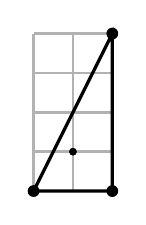
\begin{tikzpicture}[scale=0.5]
			\draw[black!30!white,line width=1pt] (0,0) grid (2,4);
			\draw[line width=1.2pt] (0,0) -- (2,0) -- (2,4) -- cycle;
			\fill (0,0) circle (0.15) (1,1) circle (0.1) (2,4) circle (0.15) (2,0) circle (0.15);
			\end{tikzpicture}
		\end{center}
		The necessary condition for SOS is fulfilled. It's twice a lattice polytope and the coefficient corresponding to the vertices are positive. Consider the half of the Newton polytope: 
		\begin{center}
			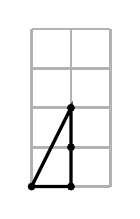
\begin{tikzpicture}[scale=0.5]
			\draw[black!30!white,line width=1pt] (0,0) grid (2,4);
			\draw[line width=1.2pt] (0,0) -- (1,0) -- (1,2) -- cycle;
			\fill (0,0) circle (0.1) (1,0) circle (0.1) (1,1) circle (0.1) (1,2) circle (0.1);
			\end{tikzpicture}
		\end{center}
		So, we know that we can choose $m(X)$ consisting of monomials with the vector exponents $00,10,11,12$. So, we'll need to come up with a matrix $Z$ whose rows and columns are indexed by $00,10,11,12$, and there will be linear equalities for the entries of $Z$ derived from the condition $f=m(X)^\top Z m(X)$. Let's see what results we obtain when we add two vectors from the list $00,10,11,12$: 
		\begin{align*}
			(0,0) & = (0,0) + (0,0)
			\\ (1,0) & = (0,0) + (1,0)
			\\ (1,1) & = (0,0) + (1,1)
			\\ (1,2) & = (0,0) + (1,2)
			\\ (2,0) & = (1,0) + (1,0)
			\\ (2,1) & = (1,0) + (1,1)
			\\ (2,2) & = (1,1) + (1,1) = (1,0) + (1,2)
			\\ (2,3) & = (1,1) + (1,2)
			\\ (2,4) & = (1,2) + (1,2)
		\end{align*}
		(the above equalities can also be nicely illustrated in a picture showing  $c= \frac{1}{2} (a+b)$ with $a,b$ being even integer vectors).
		So, we see that almost all entries of $Z$ are actually determined uniquely by $f$. The only entries, where we cannot guarantee uniqueness are $z_{11,11}$ and $z_{10,12}$. So, we will denote $z_{10,12}$ by $-t$ and then we see that one needs to have $z_{11,11}= 2t $, because of the relation $z_{11,11} + 2 z_{10,12} = 0$. 
		\[
		Z:=\bordermatrix{
			& 00 & 10 & 11 & 12
			\cr 00 & 2 & 0 & -2 & 0
			\cr 10 & 0 & 1 & 0 & -t
			\cr 11 & -2 & 0 & 2t & 0
			\cr 12 & 0 & -t & 0 & 1
		}
		\]
		Our matrix follows a checkerboard template. If we order the vector monomials differently, we'll get a block structure: 
		\[
		Z:=\bordermatrix{
			& 00 & 11 & 10 & 12
			\cr 00 & 2 & -2 & 0 & 0
			\cr 11 & -2 & 2t & 0 & 0
			\cr 10 & 0 & 0 & 1 & -t
			\cr 12 & 0 & 0 & -t & 1
		}
		\]		
		For the positive semidefiniteness both blocks should be positive semidefinite. The positive semidefiniteness of $2 \times 2$ blocks can be expressed through minors easily. And so, we easily convince ourselves that the matrix is PSD only for one choice of $t$, which is $t=1$. That is, our $Z$ turns out to be unique
		\[
		Z:=\bordermatrix{
			& 00 & 11 & 10 & 12
			\cr 00 & 2 & -2 & 0 & 0
			\cr 11 & -2 & 2 & 0 & 0
			\cr 10 & 0 & 0 & 1 & -1
			\cr 12 & 0 & 0 & -1 & 1
		}
		\]		
		The two blocks are rank one matrices. So, they can be written as a product of a vector times its transposed. Out of this decomposition, we'll come to a respective decomposition of the whole $Z$. 
		\[
		Z:=2 \cdot \bordermatrix{
			& 
			\cr 00 & 1 
			\cr 11 & -1 
			\cr 10 & 0 
			\cr 12 & 0 
		}
	\bordermatrix{
		& 00 & 11 & 10 & 12
		\cr  & 1 & -1 & 0 & 0
	}
	+ 
\bordermatrix{
	& 
	\cr \textcolor{red}{00} & 0
	\cr \textcolor{red}{11} & 0 
	\cr \textcolor{red}{10} & 1 
	\cr \textcolor{red}{12} & -1 
}
\bordermatrix{
	& \textcolor{red}{00} & \textcolor{red}{11} & \textcolor{red}{10} & \textcolor{red}{12}
	\cr  & 0 & 0 & 1 & -1
}		\]		
		Now, we can write down the SOS decomposition of $f$
		\[
			f = 2 (1- X_1X_2)^2 + (X_1 - X_1 X_2^2)^2.
		\]
\end{solution}


\subsection{Unconstrained univariate POP gets reduced to SDP}

One of the simplest possible cases is the case $n=1$. By the following exercise, we show that univariate global polynomial optimization can be reduced to semidefinite optimization. Some might think that univariate POP is trivial. This is not quite true, there are a number of publications on the univariate case; see related publications \cite{MR3385951,MR2736359,MR2742714} on computing the real roots of real univariate polynomials.



\begin{exercise}
	\label{univariate}
	Show the following: 
	\begin{enumerate}[(a)]
		\item A univariate polynomial $f \in \R[X]$ is non-negative if and only if $f$ is SOS. 
		\item If a univariate polynomial $f \in \R[X]$ is non-negative, it is a sum of at most two squares. 
	\end{enumerate}
\end{exercise}
\begin{solution}
	For (a), we need to show that every non-negative polynomial $f \in \R[X]$ is SOS (the converse is clear) and (b) is \blue{a refinement} of (a). So, we only prove (b). Assume $f \ne 0$. The coefficient at the highest degree monomial of $f$ is strictly positive (because $f(x) \to +\infty$ as $x\to +\infty$). After rescaling, we can assume that the coefficient at the highest order monomial of $f$ is $1$. Since $f$ is real, the complex roots of $f$ come in conjugate pairs. Thus, from the complex factorization of $f$, we can derive the representation 
	\[
		f = \prod_{s \in S} (X-a_s)^{k_s} \prod_{j \in J} ( (X-b_j)^2  + c_j^2)^{l_j}
	\]
	where $S$ and $J$ are finite index sets, $a_s, b_j \in \R, c_j \in \R \setminus \{0\}$ and $k_s,l_j \in \N$. Clearly, each $k_s$ is even (as otherwise $f$ would change sign at the root $a_s$). Thus the product over $s \in S$ is a square of a polynomial and thus also a sum of two squares (add the trivial square $0^2$). Each term $(X-b_j)^2 + c_j^2$ is a sum of squares of two polynomials $(X-b_j)$ and $c_j$. Thus, $f$ can be written as $f = (f_1^2 + g_1^2 ) \cdots (f_t^2 + g_t^2)$ for some finitely many polynomials $f_1,\ldots,f_t,g_1,\ldots,g_t \in \R[X]$. We can now modify the above representation iteratively, decreasing $t$ by one in each iteration. For this, use the following formula which shows that the product of sums of two squares can be converted into a sum of two squares
	\[
		(a^2 + b^2) (c^2 + d^2) = (ac - bd)^2 + (ad + bc)^2,
	\]
	valid for all $a,b,c,d$. To convince yourself in the validity of the formula you may introduce two complex numbers $z = a + i b$ and $w = c + i d$, where $i=\sqrt{-1}$. Then you can easily see that the formulas is just the equality $|z|^2 |w|^2 = |zw|^2$ involving the absolute values of $z, w$ and $zw$. 
\end{solution}

\subsection{The case of degree two gets reduced to linear algebra} 

\begin{lemma} \label{homogenization}
	Let $f \in \R[X_1,\ldots,X_n]$ be a polynomial of degree at most $2d$. Then
	\begin{enumerate}[(a)]
		\item \label{hom} $g:=X_0^{2d} f(X_1/X_0,\ldots,X_n/X_0) \in \R[X_0,\ldots,X_n]$ is a homogeneous polynomial of degree at most $2d$ with $g(1,X_1,\ldots,X_n) = f(X_1,\ldots,X_n)$.
		\item \label{nonneg:pol:hom} $f \ge 0$ on $\R^n$ $\Leftrightarrow$ $g \ge 0$ on \blue{$\R^{n+1}$} $\Leftrightarrow$ $g \ge 0$ on a sphere in $\R^{n+1}$ with the center at the origin.
		\item \label{sos:pol:hom} $f$ is SOS $\Leftrightarrow$ $g$ is SOS of homogeneous polynomials. 
	\end{enumerate}
\end{lemma}
\begin{proof}
	\eqref{hom} and \eqref{nonneg:pol:hom} are quite clear. 
	
	\eqref{sos:pol:hom}: if $f = f_1^2 + \cdots + f_r^2$, then by Proposition~\ref{newton:SOS} the degrees of $f_i$'s are at most $d$. Then $g = g_1^2 + \cdots + g_r^2$, where $g_i = X_0^d f_i(X_1/X_0,\ldots,X_n/X_0)$ is a homogeneous polynomial of degree $d$. Conversely, if $g= g_1^2  + \cdots + g_r^2$ for some homogeneous polynomials $g_1,\ldots,g_r$, then $f=f_1^2 + \cdots + f_r^2$ with $f_i = g_i(1,X_1,\ldots,X_n)$. 
\end{proof}

Quadratic optimization is a classical topic in numerical linear algebra. It is well-known there that solving a linear system $A x = b$ for a symmetric positive definite matrix $A$ is equivalent to the minimization of $f(x):=\frac{1}{2} \sprod{A x}{x} - \sprod{b}{x}$, and that there are methods employing this equivalence (e.g., conjugate gradients). 

\begin{exercise}
	\label{degree:two}
	If $f \in \R[X]$ is of degree two, then $f$ is non-negative if and only if $f$ is SOS. 
\end{exercise}
\begin{solution}
	Using an additional variable $X_0$, we can turn $f(X_1,\ldots,X_n)$ into a homogeneous degree-two polynomial $h(X_0,X_1,\ldots,X_n)=X_0^2 f(X_1 / X_0,\ldots,X_n / X_0 )$. 
	
	If $f$ is non-negative, then its homogenization $h$, too, is non-negative. We can write $h$ as 
	\[ h = \bar{X}^\top A \bar{X}, \] where $A \in \cS^{n+1}$ and $\bar{X} = (X_0,X_1,\ldots,X_n)^\top$. Since $h$ is non-negative, $A$ is psd. Writing $A$ as a sum of rank-one psd matrices (see Exercise~\ref{sdp:sum:rank:1}), we get the claim. 
\end{solution}


\subsection{Non-negativity vs. SOS: multivariate counterexamples} 

It turns out that for every $n \ge 2$, there exist non-negative $n$-variate polynomials which are not SOS. 

\goodbreak
\begin{proposition}
	\label{motzkin}
	For the two-variate degree-six polynomial 
	\[
		f = 1 -3 X_1^2 X_2^2 + X_1^2 X_2^4 + X_1^4 X_2^2
	\]
	the following hold:
	\begin{enumerate}[(a)]
		\item $f$ is non-negative.
		\item $f$ attains the value $0$.
		\item $f$ is not SOS. 
		\item $f-y$ is not SOS for every $y \in \R$. 
	\end{enumerate}
\end{proposition}
\begin{proof}	
	(a): The inequality for the arithmetic geometric mean of three values yields
	\[
		\frac{1 + x_1^2 x_2^4 + x_1^4 x_2^2}{3} \ge \sqrt[3]{ 1 (x_1^2 x_2^4) (x_1^4 x_2^2)} = x_1^2 x_2^2
	\]
	for all $x_1,x_2 \in \R$. This shows that $f \ge 0$ on $\R^2$. 
	
	(b): When $x_1, x_2 \in \{-1,1\}$, the value $0$ is attained, because we take the arithmetic and the geometric mean of three ones. 
	
	(c):  We assume the contrary, $f=f_1^2 + \cdots + f_r^2$ for some polynomials $f_1,\ldots,f_r \in \R[X]$ and get a contradiction using  Proposition~\ref{newton:SOS}. The Newton polytope of $f$ is $2 P$, where $P$ is a triangle with vertices $(0,0), (1,2)$ and $(2,1)$. 
	
	\begin{center}
		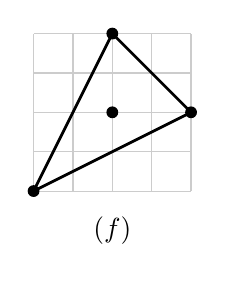
\begin{tikzpicture}[scale=0.5]
		\draw[black!20!white] (0,0) grid (4,4);
		\draw[line width=1pt] (0,0) -- (2,4) -- (4,2) -- cycle;
		\foreach \x/\y in {0/0,2/2,2/4,4/2} {
			\fill (\x,\y) circle (0.15);
		}
		\node at (2,-1) {$\newt(f)$};
		\end{tikzpicture}
		\hspace{10ex}
		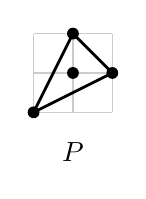
\begin{tikzpicture}[scale=0.5]
		\draw[black!20!white] (0,0) grid (2,2);
		\draw[line width=1pt] (0,0) -- (1,2) -- (2,1) -- cycle;
		\foreach \x/\y in {0/0,1/1,1/2,2/1} {
			\fill (\x,\y) circle (0.15);
		}
		\node at (1,-1) {$P$};
		\end{tikzpicture}
	\end{center}
	
	There are not so many integer points in this triangle: apart from the vertices, it is only the point $(1,1)$. Since $\newt(f_j) \subseteq P$ for every $j \in [r]$, we get 
	\[
		f_j = \sum_{\alpha \in E} c_{j,\alpha} X^\alpha,
	\]
	where 
	\[
		E:= \{(0,0),(1,2),(2,1),(1,1)\}.
	\]
	For the sum of squares we have 
	\[
		f = \sum_{j=1}^r f_j^2 = \sum_{j=1}^r \blue{\sum_{(\alpha, \beta) \in E^2} c_{j,\alpha}c_{j,\beta} X^{\alpha + \beta}. }
	\]
	Thus, if we are interested in expressing a coefficient at the monomial $X^\gamma$ of the polynomial through the coefficients of the $f_j$'s, we need to check for representations $\gamma = \alpha + \beta$ with $\alpha, \beta \in E$. It \blue{is convenient} to view the latter equation as an equation for the midpoints of segments with \blue{points} in $2 E$, by rewriting it as $\gamma = \frac{1}{2}(2 \alpha + 2 \beta)$, where $2 \alpha, 2 \beta \in E$. 
	\begin{center}
		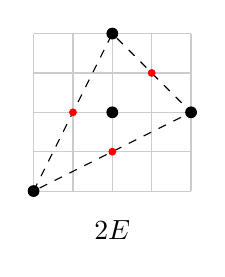
\begin{tikzpicture}[scale=0.5]
		\draw[black!20!white] (0,0) grid (4,4);
		\draw[dashed] (0,0) -- (2,4) -- (4,2) -- cycle;
		\foreach \x/\y in {0/0,2/2,2/4,4/2} {
			\fill (\x,\y) circle (0.15);
		}
		\foreach \x/\y in {1/2,2/1,3/3} {
			\fill[red] (\x,\y) circle (0.1);
		}
		\node at (2,-1) {$2 E$};		
		\end{tikzpicture}
	\end{center}	
	One immediately sees that the only way to obtain the representation $(2,2) = \frac{1}{2} ( 2 \alpha + 2 \beta)$ is by taking both $\alpha$ and $\beta$ equal to $(1,1)$. This shows that $\sum_{j=1}^r c_{j,(1,1)}^2$ is the coefficient of $f$ at the monomial $X^\gamma$ with $\gamma = (2,2)$. But this coefficient is $-3$, and we arrive at $-3 \ge 0$, which is a contradiction. 
	
	(d): The proof of (c) can be used without any changes if $y \ne 1$. If $y=1$, then the Newton polytope of $f$ gets different, because the constant term disappears. In this case, however we see that $f -y $ is not SOS, because $f$ attains negative values. We get $f-1 = X_1^2 X_2^2 (-3 + \blue{X_1^2} + X_2^2)$. So $\blue{f(x_1,x_2) - 1} < 0$ if $x_1,x_2 \in \R \setminus \{0\}$ and the distance of $(x_1,x_2)$ to $(0,0)$ is strictly less than $\sqrt{3}$. 
\end{proof}

\begin{itemize}
	\item \blue{Proposition~\ref{motzkin}}(c) was originally proved without any explicit use of Newton polytopes; see, for example, \cite{Marshall:2008}. The use of Newton polytopes is helpful as it makes the proof idea very clear.
	\item Another useful thing we learn from the proof that uses Newton polytopes is that there is a generalization of the notion of vertex in the world of lattice polytopes (or one can call the world of lattice convex sets, if you like). What we actually proved is the following: if $f$ is SOS and $2P = \blue{\newt(f)}$, then we can define $E = P \cap \Z^n$ and consider the set $2 E$. The set $2E$ is the set of all points of the lattice $(2\Z)^n$ that belong to $\blue{\newt(f)}$. This set $2 E$ has `vertices' (which are the vertices of $\blue{\newt(f)}$) and `generalized vertices', which are points $\gamma$ that cannot be written as $\gamma = \frac{1}{2} (2 \alpha + 2 \beta)$ with $\alpha, \beta \in E$ and $\alpha \ne \beta$. We have essentially shown that if $f$ is SOS and $\gamma$ is a generalized vertex of $2 E$, then the coefficient of $f$ at $X^\gamma$ must be non-negative.
\end{itemize}


Our SDP approach to lower-bounding $f$ does not work at all for $f$ in \blue{Proposition~\ref{motzkin}}, even though $f$ is pretty simple: only two variables and degree six. This $f$ is called the \emph{Motzkin polynomial}. It was discovered by Motzkin. Hilbert was the first to show (in 1888) that SOS is not always equivalent to non-negativity but he didn't give any explicit examples. An explicit example (Motzkin polynomial) was discovered much later, in 1965.

If we allow three variables, we can find a similar polynomial of degree four.

\begin{exercise}
	\label{choi:lam:exer}	
	Show that the following three-variate degree-four polynomial 
	\[
		f = 1 + X_1^2 X_2^2 + X_2^2 X_3^2 + X_1^2 X_3^2 - 4 X_1 X_2 X_3
	\]
	is non-negative, but not SOS. 
\end{exercise} 
\begin{solution}
	To see non-negativity, one can again use the inequality for the geometric and the arithmetic mean: observe that for the four exponent vectors 
	\[
		(0,0,0), (2,2,0),(0,2,2), (2,0,2), (1,1,1)
	\]
	the last one is the arithmetic mean of the remaining ones. 
	For showing that $f$ is not SOS, we can use the Newton polytope of $f$. It can be represented as $2 P$, with $P = \conv( (0,0,0), (1,1,0), (0,1,1), (1,0,1) )$. Here, $P$ is a simplex, and apart from its vertices, there are no other integer points in $P$. If we could write $f$ as $f= f_1^2 + \cdots + f_r^2$, then we had $\newt(f_j) \subseteq P$. Due to the observation about $P$,  $f_j^2$ does not contain the monomial  $X_1 X_2 X_3$. But $f$ does contain this monomial, so we get a contradiction. 
\end{solution}

The polynomial from the previous exercise is called the \emph{Choi-Lam-polynomial}. 

Here are two exercises that illustrate that passing from the dual problem \eqref{unconst:POP:dual:eq} to its SOS-relaxation \eqref{unconst:POP:dual:SOS:eq} one can get a finite positive gap. 

\begin{exercise}
	\label{parrilo:example}
	Consider the homogenization
	\[
	h(X_1,X_2,X_3) := X_3^6 -3 X_1^2 X_2^2 X_3^2 + X_1^2 X_2^4 + X_1^4 X_2^2
	\]
	of the Motzkin polynomial (it is called the \emph{Motzkin form}). Show that 
	\begin{enumerate}[(a)]
		\item $f = h(X_1,1,X_3)$ is non-negative, 
		\item $f$ is not SOS, but 
		\item $h(X_1,1,X_3) +c$ is SOS for some $c \in \R$. 
	\end{enumerate}
\end{exercise}
\begin{solution}
	The examples can be found in \cite[Example~7.2]{Parrilo:2003}.
	\begin{enumerate}[(a)]
	\item Since the Motzkin polynomial $h(X_1,X_2,1)$ is non-negative, also \blue{by Lemma~\ref{homogenization}}, $h(X_1,X_2,X_3)$ is non-negative. Since $h$ is non-negative, then also $f$ is non-negative. 
	\item If $f$ were SOS, then by homogenization of the SOS-representations, we'd get that $h$ is SOS. But then also the Motzkin polynomial $h(X_1,X_2,1)$ would be SOS, which is a contradiction. 
	\item We have
	\[
		f=X_3^6 - 3 X_1^2 X_3^2 + X_1^2 + X_1^4 .
	\]
	The disturbing term here is $- 3 X_1^2 X_3^2$, because its coefficient is negative. We get rid of this term using 
	\[
		X_1^4  - 3 X_1^2 X_3^2 = (X_1^2 - \frac{3}{2} X_3^2)^2 - \frac{9}{4} X_3^4.
	\]
	Thus, we arrive at
	\[
		f = \bigl(X_3^6 - \frac{9}{4} X_3^4 \bigr) + (X_1^2 - \frac{3}{2} X_3^2)^2 + X_1^2
	\]
	The second and third summands are squares. The first summand depends only on $X_3$ and if we add a sufficiently large constant $c$, it becomes non-negative and so SOS. One can for example check that $c=2$ will do (to see that $t^6 - \frac{9}{4} t^4 + 2 \ge 0$ for all $t \in \R$ one can distinguish between $|t| \le 1$ and $|t| \ge 1$ and estimate $t^6$ by~$t^4$ in the latter case).\qedhere
	\end{enumerate}
\end{solution}

\begin{exercise}
	Consider the Motzkin form $h$ from Exercise~\ref{parrilo:example} and the three-variate degree-twelve polynomial 
	\[
		f = (h+1)^2.
	\]
	By construction, $f$ is SOS (in fact, $f$ is a square). Show that $f-1$ is non-negative but not SOS. 
\end{exercise}
\begin{solution}
	The construction (and the solution) was communicated to me by Claus Scheiderer. 
	Observe that $h$ is not SOS. In fact, if $h$ were SOS, then also the Motzkin polynomial $h(X_1,X_2,1)$ would be SOS, which is a contradiction. One has $f - 1= (h+1)^2 - 1 = h (h+2)$, which implies that $f$ is non-negative. To see that $f-1$ is not SOS, note that $f- 1= 2 h + h^2$, where $h$ is homogeneous of degree $6$ and $h^2$ homogeneous of degree $12$. Assume the contrary, $f-1 = 2 h + h^2 = \sum_{j=1}^r g_j^2 + \cdots + g_r^2$ for some $g_1,\ldots,g_r \in \R[X]$. We introduce another indeterminate $Y$  and evaluate the above equality at $(Y X_1, Y X_2, Y X_3)$. Taking into account the homogeneity we get
	\[
		Y^6 2 h(X_1,X_2,X_3) + Y^{12} h(X_1,X_2,X_3) = \sum_{j=1}^r g_j(Y X_1, Y X_2, Y X_3)^2. 
	\]
	Now we can view the left and the right hand sides as elements of $\R[X_1,X_2,X_3][Y]$ (univariate polynomials in $Y$ with polynomials in $X_1, X_2, X_3$ as coefficients). Since the left hand side involves only monomials $Y^6$ and $Y^{12}$,  each $g_j(Y X_1, Y X_2, Y X_3)$ can be written as $Y^3 h_j(X_1,X_2,X_3)$ plus higher order terms (for monomials $Y^4,Y^5,Y^6$). Comparing the coefficients at $Y^6$ we arrive at 
	\[
		2 h(X_1,X_2,X_3) = \sum_{j=1}^r h_j(X_1,X_2,X_3)^2.
	\]
	This contradicts the fact that $h$ is not SOS.
\end{solution}

Also other examples can be generated using the above template (using the Choi-Lam-polynomial, we can construct a four-variate polynomial of degree $8$ with similar properties).

\subsection{Equivalence of non-negativity and SOS for two-variate polynomials of degree four}

There is yet another special situation, where both the degree and the dimensions are fixed to be some specific values, in which non-negativity is equivalent to SOS. If, unlike algebraists, you are not very interested in special degrees and dimensions, you can skip this subsection or read only the formulation of Theorem~\ref{thm:ternary:quartics} below. 

We show that for two-variate polynomials of degree four, SOS is equivalent to non-negativity. The result goes back to Hilbert, but here we follow a different proof recently suggested in the literature. 

\begin{lemma}
	\label{ternary:quartics:lem}
	Let $f \in \R[X]$ be a univariate non-negative polynomial and let $q \in \R[X]$ be a strictly positive quadratic univariate polynomial. Then there exist polynomials \blue{$\eta, \xi \in \R[X]$} such that 
	\[
		f = \eta^2 + q \xi^2.
	\]
\end{lemma}
\begin{proof}
	Changing coordinates and rescaling, we can assume that $q = X^2 + 1$. Since $f$ is non-negative \blue{and w.l.o.g.~non-zero}, its degree is at least two. 
	
	If the degree of $f$ is two, we can write $f$ as $f = (X+a)^2 + b^2$ for some $a,b \in \R$. In this case $\xi^2$ must be a constant, and we show that an appropriate constant can be chosen. We want the constant $\xi$ to be chosen in such a way that $f- q\xi^2$ is a square of a polynomial. Let's compute the coefficients of $f-q \xi^2$:
	
	\begin{align*}
		f - q \xi^2 & = (X+a)^2 + b^2 - (X^2 + 1) \xi^2 
		\\ & = (1-\xi^2) X^2 + 2 a X + a^2 + b^2 - \xi^2.
	\end{align*}
	For $f-q \xi^2$ to be a square of a real polynomial, it is necessary that the coefficient at $X^2$ is non-negative. Thus, we should look for $\xi$ satisfying  $\xi^2 \le 1$. Under this condition, the polynomial $f- q \xi^2$ is a square of a linear polynomial if both its roots coincide, which can be expressed as the discriminant being equal to zero. The discriminant of $f - q \xi^2$ is 
	\[
		\Delta := 4 a^2 - 4 (1-\xi^2) (a^2 + b^2 -\xi^2).
	\] 
	As $\xi^2$ moves from $0$ to $1$, the discriminant $\Delta$ gets changed from $- 4 b^2$ to $4 a^2$. So there is a choice of $\xi^2$ with $\Delta=0$. 
	
	If the polynomial $f$ is of degree larger than two, we use induction. Factorize $f$ as $f=f_1 f_2$, where $f_1$ and $f_2$ are non-constant non-negative polynomials. Such a factorization exists, because $f$ is a product of linear terms and quadratic polynomials (by the fundamental theorem of algebra).
	
	Using the induction assumption for $f_1$ and $f_2$, write each of them in the desired form $f_j = \eta_j^2 + q \xi_j^2$. This gives 
	\begin{align*}
		f & = (\eta_1^2 + q \xi_1^2) (\eta_2^2 + q \xi_2^2) .
	\end{align*}
	We will convert the expression above to the desired form $ f= \eta^2 + q \xi^2$. This can be done just by defining the right $\eta$ and $\xi$ and leaving the comparison of the two expressions as a routine verification. But it would probably be better to have a derivation that is easy to track. So, we'll be using a formal root $\sqrt{q}$ of $q$ (which can be rigorously introduced algebraically) and we will use the root of $-1$, defined by $i^2 = -1$. With this additional objects, we can essentially use the formula $|z_1 z_2| = |z_1| \cdot |z_2|$ for the absolute value of the product of complex numbers $z_1, z_2 \in \compl$ as follows: 
	\begin{align*}
		f & = \bigl(\eta_1^2 + ( \sqrt{q} \xi_1)^2 \bigr) \bigl(\eta_2^2 + (\sqrt{q} \xi_2)^2 \bigr) 
		 \\ & = \bigl | \eta_1 + i \sqrt{q} \xi_1 \bigr|^2 \bigl| \eta_2 + i \sqrt{q} \xi_2 \bigr|^2
		 \\ & = \bigl | (\eta_1 + i \sqrt{q} \xi_1) (\eta_2 + i \sqrt{q} \xi_2) \bigr|
		 \\ & = \bigl| \eta_1 \eta_2 - q \xi_1 \xi_2 + i (\sqrt{q} \xi_1 \eta_2 + \sqrt{q} \xi_2 \eta_1 ) \bigr|
		 \\ & = (\underbrace{\eta_1 \eta_2 - q \xi_1 \xi_2}_{=:\eta})^2 + q ( \underbrace{\xi_1 \eta_2 + \xi_2 \eta_1}_{=:\xi})^2.
	\end{align*}
	This gives a desired expression $ f= \eta^2 + q \xi^2$. In case, one does not believe that the intermediate steps in this calculation have a rigorous mathematical meaning, one could just check that 
	\[
		(\eta_1^2 + q \xi_1^2) (\eta_2^2 + q \xi_2^2) = (\eta_1 \eta_2 - q \xi_1 \xi_2)^2 + q (\xi_1 \eta_2 + \xi_2 \eta_1)^2,
	\]
	is true, which is nothing but checking a polynomial identity. 
\end{proof}

Having this lemma, we can now prove the following. 

\begin{theorem}[Hilbert]
	\label{thm:ternary:quartics}
	Every non-negative two-variate polynomial of degree at most four is SOS. 
\end{theorem}
\begin{proof}
	For the case $n=2, d=4$, the following proof can be given, which is obtained by simplifying the proof in \cite{Pfister:Scheiderer:2012} (see also a related proof in \cite[Prop.~6.3.4]{Bochnak:Coste:Roy:1998}). 
	
	We'll work with homogeneous polynomials in three indeterminates here and we prefer to denote these indeterminates as $X, Y, Z$ in this proof. 
	
	A non-negative two-variate polynomial $g \in \R[X,Y]$ of degree at most four can be homogenized to the three-variate non-negative polynomial $f \in \R[X,Y,Z]$ of degree~$4$ via
	\[
		f(X,Y,Z) := Z^4 g(X/Z,Y/Z).
	\]
%	In terms of exponent vectors, the homogenization from $g$ to $f$ goes by replacing an exponent vector in $\Z_+^2$ with an exponent vector in $\Z_+^3$ by appending a new component so that the sum of the components of the new exponent vector is $4$.
\blue{We have seen in Lemma~\ref{homogenization}}, that whenever $g \ge 0$ on $\R^2$, the homogenization $f$ is non-negative on $\R^3$. Using this operation, we replace the study of arbitrary non-negative polynomials of degree at most $4$ in $2$ indeterminates by a study of homogeneous non-negative polynomials of degree \blue{at most} $4$ in $3$ indeterminates. Let's denote by $C$ the cone of these polynomials 
	\[
		C:= \setcond{ f \in \R[X,Y,Z]}{f \ \text{homogeneous}, f \ge 0 \ \text{on} \ \R^3, \ \blue{\deg(f) \leq 4}}.
	\]
	Clearly, the cone is finite-dimensional, convex and closed. It is also not hard to see that the cone is pointed. To see this, we need to consider $f \in C \cap (-C)$. Such $f$ satisfies $f=0$ on $\R^3$. But, since our underlying domain of coefficients is $\R$,  the latter implies that $f$ is a zero polynomial. Let's recall that a zero polynomial is a polynomial, whose all coefficients are zero. Thus, out of $f(x,y,z) =0$ for all $(x,y,z) \in \R^3$ one needs to conclude that all coefficients of $f$ are zero. This is not particularly difficult but still requires a small argument (we leave the verification as an exercise). 
	
	We know from convexity theory that every vector in a closed pointed convex cone is a sum of finitely many vectors that lie on the extremal rays of the cone. Thus, it suffices to show the assertion for $f$ lying on the extremal ray of $C$.	Consider the unit sphere 
	\[
		S := \setcond{(x,y,z) \in \R^3}{x^2 + y^2 + z^2 = 1}.
	\]
	Due to the homogeneity, the condition $f \ge 0$ on $\R^3$ for homogeneous polynomials can be expressed as $f \ge 0$ on $S$. If a homogeneous polynomial $f$ is strictly positive on $S$, then $f$ would lie in the interior of $C$, as one would have $f+ h \ge 0$ on~$S$ for \blue{every} homogeneous polynomial~$h$ with sufficiently small coefficients. Polynomials in the interior of $C$ are not \blue{contained} in the extremal rays of $C$. So, we can assume that $f \in C$ is equal to zero for at least one $(x,y,z) \in S$. Applying a rotation of $\R^3$ around $(0,0,0)$ we can assume that $f(0,0,1) = 0$. 
	
	We can interpret $\R[X,Y,Z]$ as $\R[X,Y][Z]$ and correspondingly write $f$ as 
	\[
	f(X,Y,Z) = f_0 Z^4 + f_1 Z^3 + f_2 Z^2 + f_3 Z + f_4,
	\] 
	where $f_j \in \R[X,Y]$ is homogeneous of degree $j$, or the zero polynomial. Since $f(0,0,1)=0$, we get $f_0=0$. But then we can also see that $f_1 = 0$. A rigorous way to see this is as follows: We have 
	\[
		0 \le z^{-3} f(x,y,z) = f_1(x,y)  + f_2(x,y) z^{-1} + f_3 z^{-2} \blue{ + f_4 z^{-3}} \to f_1(x,y), \quad \text{as} \ z \to +\infty.
	\]
	This shows $f_1(x,y) \ge 0$, where $f_1$ is a homogeneous polynomial $f_1$ of degree $1$ or equal to $0$. This implies $f_1=0$. 

	Thus, we get
	\[
		f(X,Y,Z) = f_2(X,Y) Z^2 + f_3(X,Y) Z + f_4(X,Y).
	\]
	That is, out of the assumption $f(0,0,1)$ we came to the conclusion that the degree of $f$ with respect to $Z$ is at most two. We proceed by looking at the properties of the `coefficient polynomials' $f_2$ and $f_3$ and $f_4$. Clearly, $f_4 \ge 0$ on $\R^2$ since $f_4(X,Y)= f(X,Y,0)$. On the other hand we have $f_2 \ge 0$ on $\R^2$, which can be shown using an argument similar to the one that we used to show $f_1 \ge 0$ above. We distinguish cases according to the properties of the quadratic form $f_2(X,Y)$.
	
\smallskip
	\emph{Case~1:}	$f_2(X,Y)=0$. Then $f(X,Y,Z) = f_3(X,Y) Z + f_4(X,Y)$ and we must have $f_3 = 0$. Indeed, if we did have $f_3 \ge 0$, then there would be a point $(x,y) \in \R^2$ with $f_3(x,y) \ne 0$. Then $f(x,y,Z)$ is a polynomial of degree one, and we know that a polynomial of degree one cannot be non-negative, which is a contradiction. Hence $f(X,Y,Z) = f_4(X,Y)$. Since $f_4(X,Y) \ge 0$ on $\R^2$, we conclude that $f_4(X,1) \ge 0$ is non-negative on $\R$. \blue{In view of Exercise~\ref{univariate}}, we can write $f_4(X,1)$ as a sum of squares $f_4(X,1) = \sum_{j=1}^r g_j(X)^2$ of polynomials $g_j$ of degree at most two \blue{(actually we could choose $r=2$)}.  Homogenizing this we have 
	\[
		\blue{f(X,Y,Z) = }f_4(X,Y) = Y^4 f_4(X/Y,1) = \sum_{j=1}^r (Y^2 g_j(X/Y))^2,
	\]
	where $Y^2 g_j(X/Y)$ is a homogeneous polynomial of degree two. 	

\smallskip
	\emph{Case~2:} The set of zeros of $f_2$ is a one-dimensional linear space. Then $f_2 = l^2$ for some non-zero linear form $l \in \R[X,Y]$. 	
	\[
		f = l^2 Z^2 + f_3 Z + f_4 .
	\]
	Whenever $(x,y) \in \R^2$ is such that $l(x,y)=0$ holds we get \blue{$f = f_3 Z  + f_4$}. But then $f_3(x,y)=0$ since otherwise, we get a contradiction to $f \ge 0$ in the same way as we did above. It follows that $l(x,y)=0$ implies $f_3(x,y)=0$. This means that~$l$ is a factor of $f_3$. Thus, we can write  $f_3 = 2 l g_2$ for some quadratic polynomial $g_2 \in \R[X,Y]$. Thus, 
	
	\[
		f = (l Z)^2 + 2 g_2 (l Z) + f_4 = (l Z + g_2)^2 + f_4 - \blue{g_2^2. }
	\]
	
	Clearly, \blue{the homogeneous bivariate polynomial} $f_4 - \blue{g_2^2}$ \blue{of degree four} is non-negative (just consider $f(x,y,z)$ for $z= - g_2(x,y) / l(x,y)$ with $l(x,y) \ne 0$, \blue{and use the continuity of polynomials}).
	\blue{Thus, by homogenizing Exercise~\ref{univariate}, it is SOS.}
	It follows that $f$ is SOS. 
	
\smallskip
	\emph{Case~3:} The set of zeros of $f_2$ is $\{(0,0)\}$. Then 
	\begin{equation}
		\label{f2:l1:l2}
		f_2 = l_1^2 + l_2^2
	\end{equation} 
	for some non-trivial linear forms $l_1, l_2 \in \R[X,Y]$. We have a polynomial $f$ which is quadratic in $Z$, and we want to extract a full square with respect to $Z$. For doing this in terms of polynomial coefficients we need to multiply $f$ with an appropriate polynomial: 
	\[
		4 f_2 f = (2 f_2 Z)^2 + 2 f_3 ( 2 f_2 Z) + 4 f_2 f_4 = (2 f_2 Z + f_3)^2 + 4 f_2 f_4 - f_3^2.
	\]
	As above, we see that $4 f_2 f_4 - f_3^2$ is non-negative. Thus, \blue{by applying Lemma~\ref{ternary:quartics:lem} after the dehomogenization $(X,Y) \mapsto (X,1)$ of all involved polynomials, and then homogenizing back again}, there exist bivariate polynomials $\xi(x,y)$ and $\eta(x,y)$ of degrees $2$ and $3$ respectively such that 
	\[
		\eta^2 + \xi^2 f_2 = 4 f_2 f_4 - f_3^2.
	\] 
	This is equivalent to
	\begin{equation}
		\label{eta:f3}
		\eta^2 +f_3^2 = f_2 (4 f_4 - \xi^2). 
	\end{equation}
	Using \eqref{f2:l1:l2}, this can be written as 
	\[
	(\eta + i f_3)(\eta - i f_3) = (l_1 + i l_2) (l_1 - i l_2)( 4 f_4 - \xi^2),
	\]
	where $i^2 = -1$. The polynomials $l_1 \pm i l_2$ have degree one and so they are prime factors. Without loss of generality, we can assume that $l_1 + i l_2$ divides $\eta + i f_3$. Hence,~$f_2$ divides 
	\[
		(\eta+ i f_3) (l_1 - i l_2) = (\eta l_1 + f_3 l_2) + i ( f_3 l_1 - \eta l_2).
	\]
	Since $f_2$ has real coefficients, $f_2$ divides both real and the imaginary part of the latter polynomial. So, the following two fractions are polynomials
	\begin{align*}
		h_1 & := \frac{f_3 l_1 - \eta l_2}{2 f_2} &  h_2 &:= \frac{\eta l_1 + f_3 l_2}{2 f_2}.
	\end{align*}
	By definition of $h_1$ and $h_2$, we have 
	\begin{align*}
		h_1^2 + h_2^2 & = \frac{1}{4 f_2^2} \Bigl((\re ((\eta+i f_3)(l_1-il_2))^2 +  (\im ((\eta+ i f_3)(l_1 - i l_2))^2 \Bigr) 
		\\ & = \frac{1}{4 f_2^2}|(\eta+ i f_3)(l_1 - i l_2)|^2 
		\\ & = \frac{1}{4 f_2^2}|\eta+ i f_3|^2 \cdot |l_1 - i l_2|^2
		\\ & = \frac{(\eta^2 + f_3^2)(l_1^2 + l_2^2)}{4 f_2^2} 
		\\ & = \frac{\eta^2 + f_3^2}{4 f_2} 
		\\ & = f_4 - \frac{1}{4} \xi^2. 
	\end{align*}
	This gives
	\begin{align}
		h_1^2 + h_2^2 & = f_4 - \frac{1}{4} \xi^2. \label{what:is:xi}
	\end{align}
	Moreover, from the definition of $h_1$ and $h_2$ we also have 
	\[
	h_1 l_1 + h_2 l_2 = \frac{f_3 (l_1^2 + l_2^2)}{2 f_2} = \frac{1}{2} f_3.
	\]
	Consequently, 
	\begin{align*}
	(\xi/2)^2 + (h_1 + l_1 Z)^2 + (h_2 + l_2 Z)^2 & \stackrel{\eqref{what:is:xi}}{=} f_4 - h_1^2 - h_2^2 + (h_1 + l_1 Z)^2 + (h_2 + l_2 Z)^2 
	\\ & = f_4 + 2 (\underbrace{h_1 l_1 + h_2 l_2}_{=\frac{1}{2} f_3}) Z + (\underbrace{l_1^2 + l_2^2}_{f_2}) Z^2 
	\\ & = f_2 Z^2 + f_3 Z+ f_4 
	\\ & = f. \qedhere
	\end{align*}
\end{proof}

\begin{exercise}
	Show that $f \in \R[X]$ is a zero polynomial if and only if $f=0$ on~$\R^n$.
\end{exercise} 

\subsection{Non-negativity vs. SOS: Summary}

\begin{theorem}
	Let $d \in \N$ and $n \in \N$. Every $n$-variate \blue{non-negative} polynomial of degree at most $2d$ is SOS if and only if one of the following conditions is fulfilled:
	\begin{enumerate}[(a)]
		\item $n=1$, or
		\item $d=1$, or
		\item $n=2, d=2$.
	\end{enumerate}
\end{theorem}
\begin{proof}
	See results and examples of this chapter (Exercise~\ref{univariate}, Exercise~\ref{degree:two}, Proposition~\ref{motzkin}, Exercise~\ref{choi:lam:exer} and Theorem~\ref{thm:ternary:quartics}).
\end{proof}



	\begin{center}
		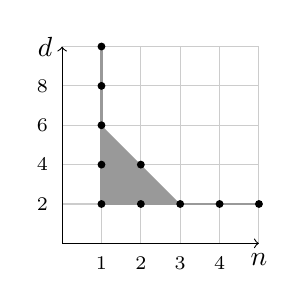
\begin{tikzpicture}[scale=0.5]
		\draw[black!20!white] (0,0) grid (5,5);
		\draw[<->] (5,0) node[below]{$n$} -- (0,0) -- (0,5) node[left]{$d$};
		\foreach \x\y in {1/2,2/4,3/6,4/8} {
			\node at (-0.5,\x) {\scriptsize $\y$};
		}
		\draw[black!40!white,line width=1pt] (1,1) -- (1,5);
		\draw[black!40!white,line width=1pt] (1,1) -- (5,1);
		\fill[black!40!white] (1,1) -- (3,1) -- (1,3) -- cycle;
		\foreach \y in {1,2,3,4} {
			\node at (\y,-0.5) {\scriptsize $\y$};
		}
		\foreach \x/\y in {1/1,2/1,3/1,4/1,5/1,1/2,1/3,1/4,1/5,2/2} {
			\fill (\x,\y) circle (0.1);
		}
		\end{tikzpicture}
	\end{center}	


\begin{remark}
	Similar characterizations were also obtained for symmetric polynomials (invariant up to permutation of variables) and for symmetric polynomials even in each variable; see \cite{choi1977old} and \cite{goel2016choi}.
\end{remark}





